% body/aicomponentdesign.tex
\chapter{AI Component Design}
\label{chap:ai-component-design}

This chapter details the design and integration of Artificial Intelligence (AI) components within the \usevar{\srsTitle} system. Understanding where AI fits into the overall workflow and the specific goals it aims to achieve is crucial for effective development and evaluation. The following sections outline the analysis, design, implementation, and evaluation considerations for the AI modules.

\section{Business Context and AI Integration}
\label{section:ai-integration-context}

\usevar{\srsTitle} tackles the complex challenge of tracking individuals across multiple camera views in environments like campuses and factories. The core task requires recognizing and associating individuals as they move between potentially non-overlapping camera fields, often amidst changing appearances, viewpoints, lighting conditions, and occlusions. This inherent complexity and real-world variability make manual tracking labor-intensive, error-prone, and difficult to address effectively with traditional rule-based programming. Artificial Intelligence is therefore central to \usevar{\srsTitle}, providing the automation necessary to significantly improve this process.

The primary AI-driven workflow resides within the system's backend processing core, orchestrated by a service like FastAPI. This workflow involves several key AI steps:
\begin{enumerate}
    \item \textbf{Person Detection:} Identifying individuals within each camera frame using high-performance detection models.
    \item \textbf{Intra-Camera Tracking:} Maintaining consistent temporary IDs for detected individuals within a single camera's view over consecutive frames, utilizing robust tracking algorithms.
    \item \textbf{Feature Extraction for Re-ID:} Generating unique appearance embeddings (features) from detected person images when necessary using discriminative feature extraction models.
    \item \textbf{Cross-Camera Re-Identification (Re-ID):} Matching these appearance embeddings across different camera views and time gaps to assign a persistent global identity, linking temporary tracks together.
    \item \textbf{Spatial Mapping:} Transforming the detected location of individuals from the camera's 2D image plane onto a unified top-down map coordinate system using geometric transformation techniques.
\end{enumerate}
These AI components perform the essential visual analysis and identity association. Figure \ref{fig:ai-architecture-overview} provides a high-level illustration of this system architecture and the integration points for these AI modules.

\begin{figure}[!htb] % Use !htb to suggest placement: here, top, bottom
    \centering
    % Use \makebox or adjust width as needed for centering wide figures
    \makebox[\textwidth][c]{
        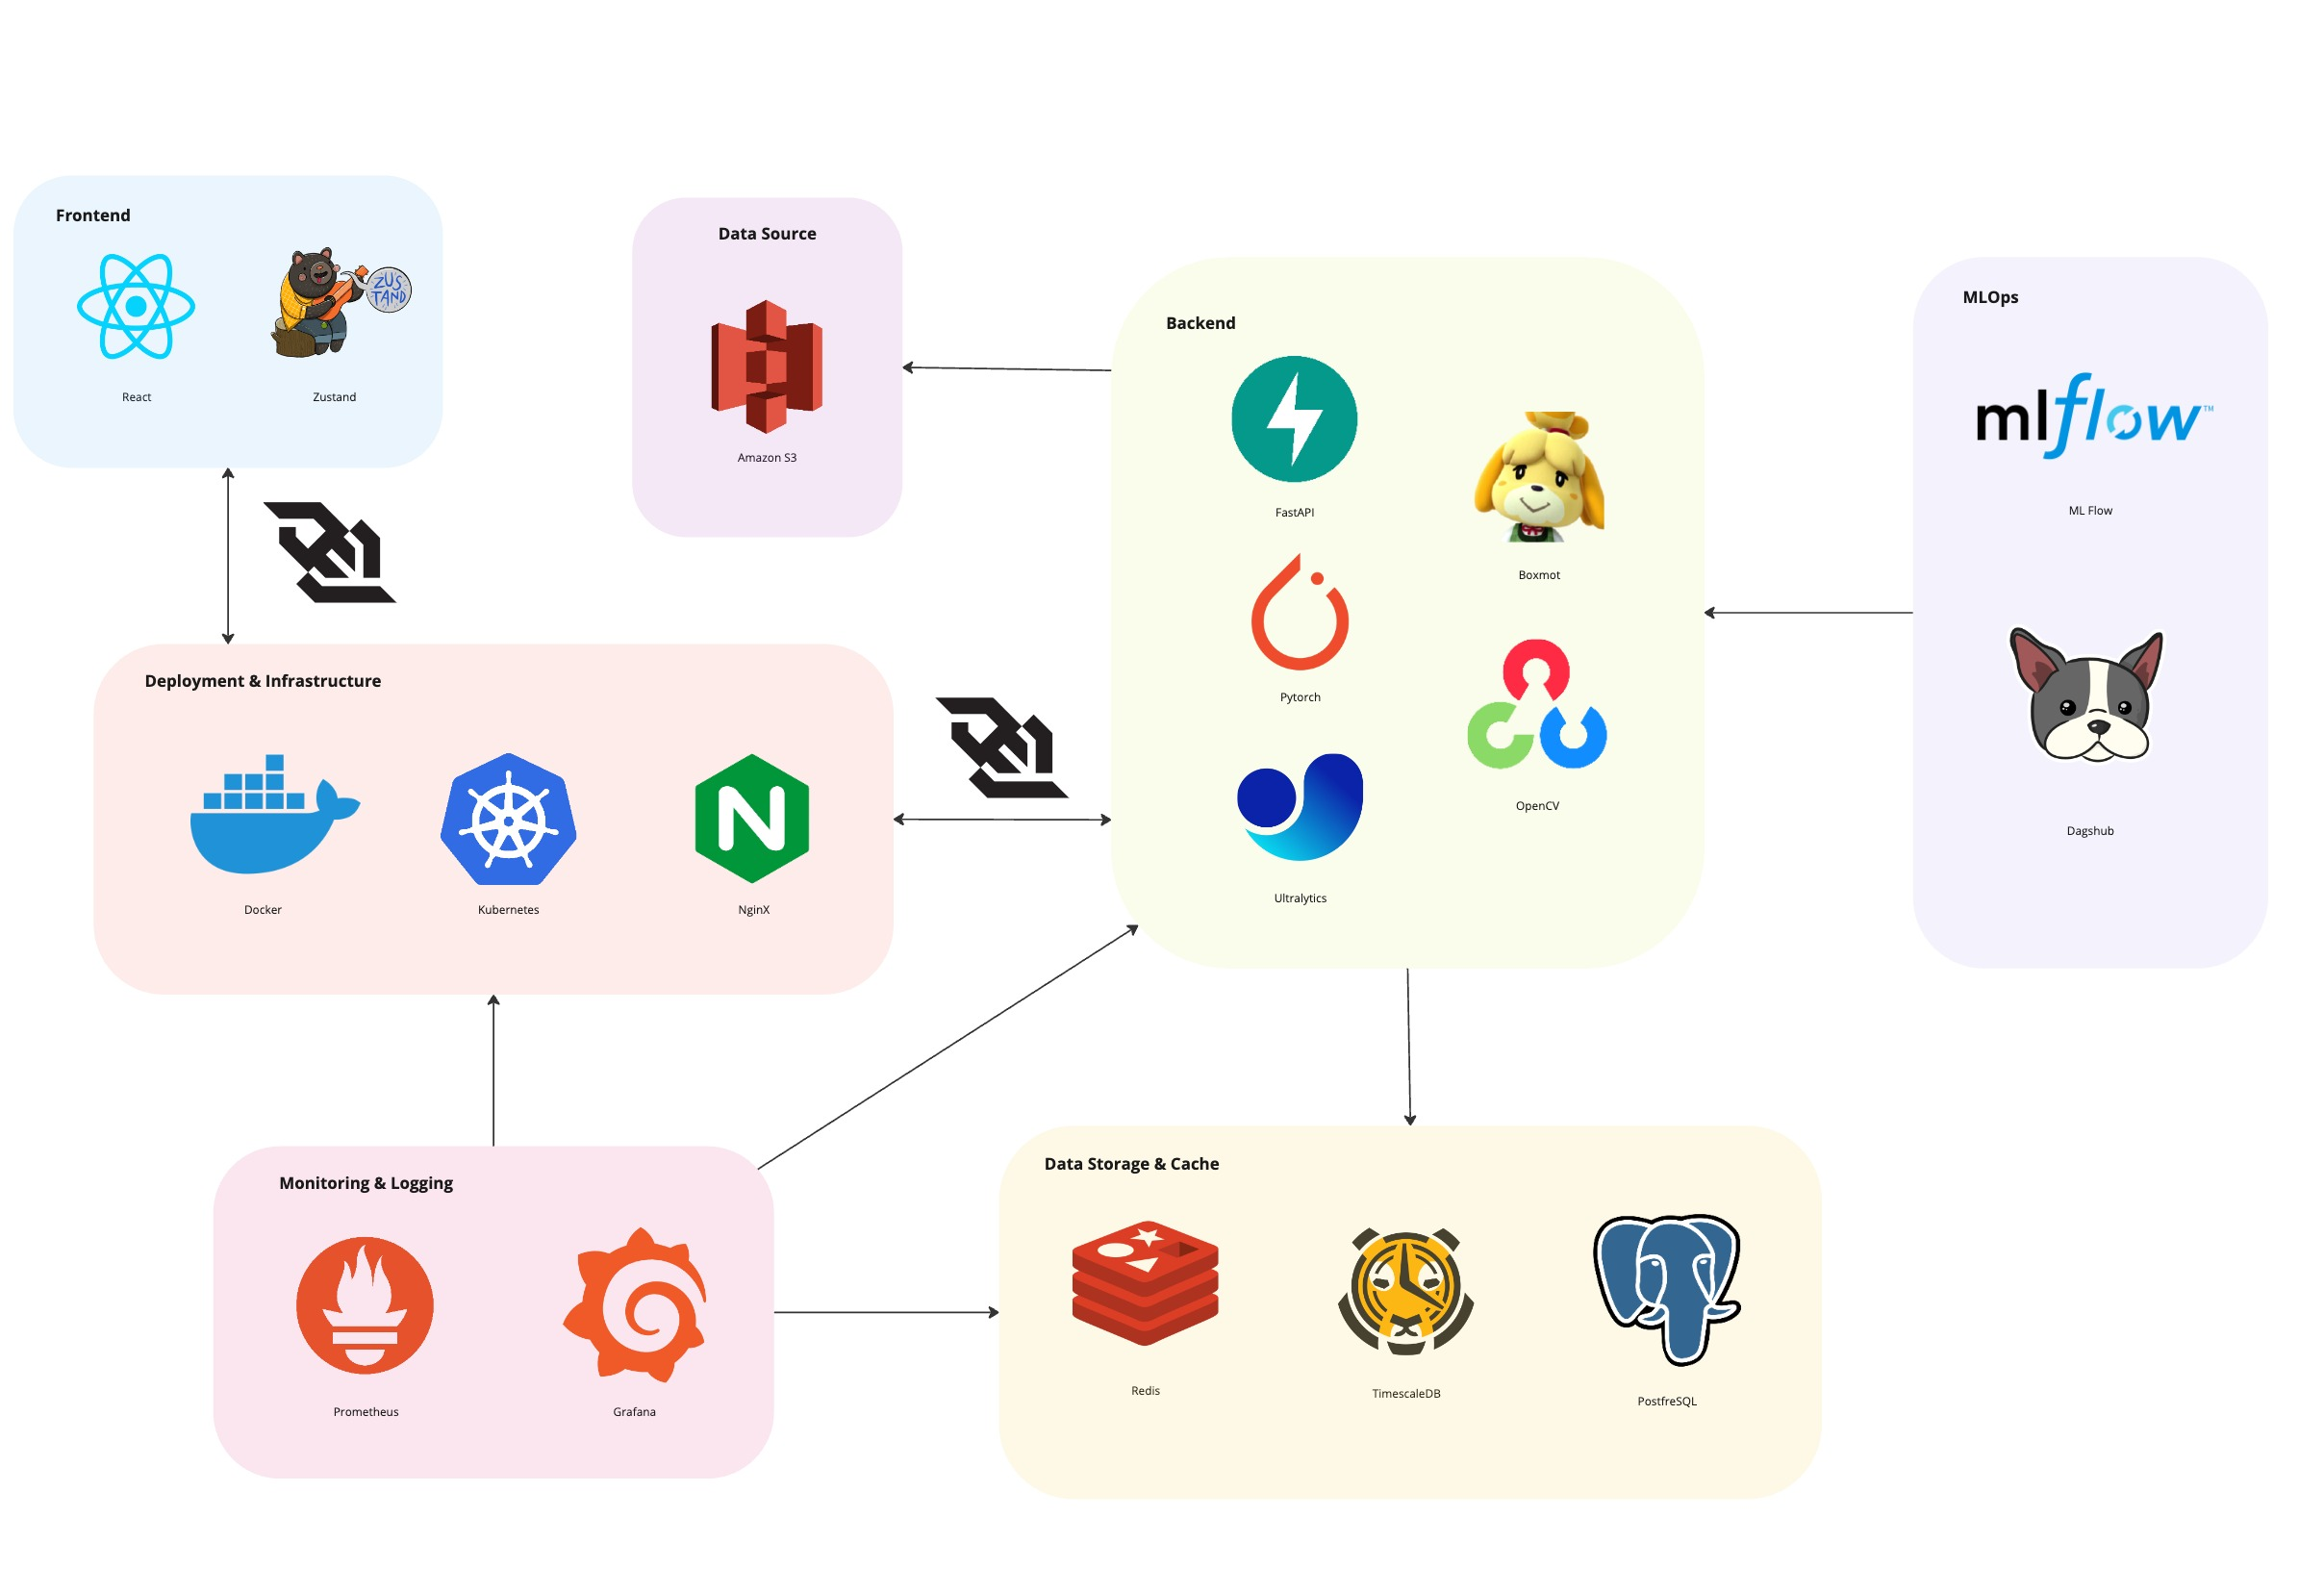
\includegraphics[width=1.0\textwidth, keepaspectratio]{jubjones/architecture.jpg}
    }
    \caption{System Architecture Overview Highlighting AI Component Integration}
    \label{fig:ai-architecture-overview}
\end{figure}
\clearpage % Ensure figure placement doesn't clash excessively with text

The justification for employing AI stems from the nature of the problem itself:
\begin{itemize}
    \item \textbf{Complexity Beyond Rules:} Recognizing and matching people under diverse visual conditions involves intricate pattern recognition that surpasses the capabilities of predefined rules. AI models excel at learning these complex patterns directly from data.
    \item \textbf{Scalability Requirement:} Manually monitoring and correlating feeds from numerous cameras is impractical. AI offers an automated solution capable of handling large data volumes and multiple camera streams simultaneously.
    \item \textbf{Adaptability to Dynamic Environments:} Real-world surveillance scenarios are constantly changing. AI, particularly deep learning, offers better generalization and adaptation to variations in lighting, crowds, and individual appearances compared to static algorithms.
    \item \textbf{Value Despite Imperfection:} Achieving flawless accuracy in cross-camera tracking is exceptionally difficult due to the inherent ambiguities and challenges (e.g., severe occlusions, drastic appearance changes). However, an AI system achieving high, albeit imperfect, accuracy still delivers significant value. It drastically reduces the manual workload for operators and provides a level of situational awareness unattainable through manual means or simpler systems. Even with occasional errors, such as false positive matches or missed detections, the system's ability to automatically correlate identities across most views aligns with the primary goal of enhancing operational efficiency and speeding up investigations. The objective is a substantial improvement over the baseline, accepting a trade-off where occasional inaccuracies are outweighed by the overall gains in automation and insight.
\end{itemize}



\section{Goal Hierarchy}
\label{section:goal-hierarchy}

Ensuring the AI components effectively contribute to the overall success of \usevar{\srsTitle} requires aligning goals across multiple levels. This hierarchical approach clarifies the purpose of each component and provides measurable targets for development and evaluation, moving from broad organizational objectives down to specific AI model performance.

\begin{itemize}
    \item \textbf{Organization Level Goals:}
        \begin{itemize}
            \item Enhance overall campus/factory safety and security posture.
            \item Improve operational efficiency for security and facility management teams.
            \item Optimize resource allocation (e.g., personnel deployment, space utilization).
            \item Reduce costs associated with manual surveillance monitoring and incident investigation time.
        \end{itemize}
        \textbf{Measurement:} Success at this level is measured via key performance indicators such as reduction in security incidents, faster incident resolution times, documented improvements in space utilization, and potential reduction in monitoring personnel hours.

    \item \textbf{System Level Goals (\usevar{\srsTitle}):}
        \begin{itemize}
            \item Provide accurate and continuous tracking of individuals across multiple, potentially non-overlapping, camera views.
            \item Maintain persistent identity of individuals even through temporary disappearances or view changes.
            \item Visualize individual movement paths clearly on a unified spatial map.
            \item Enable efficient retrospective analysis of movement patterns and incidents.
            \item Offer a reliable and usable interface for target users.
        \end{itemize}
        \textbf{Measurement:} System success is assessed through end-to-end tracking accuracy metrics (e.g., overall MOTA/IDF1 on test sequences), system uptime and reliability metrics, task completion time for key user scenarios, and user satisfaction surveys.

    \item \textbf{User Level Goals:}
        \begin{itemize}
            \item \textit{Security Officer:} Faster POI location/monitoring, efficient evidence gathering, reduced manual correlation effort. (\ref{userstory:1}, \ref{userstory:2}, \ref{userstory:5})
            \item \textit{Facility Manager:} Understanding pedestrian flow, identifying bottlenecks, optimizing space. (\ref{userstory:3})
            \item \textit{Emergency Coordinator:} Rapid location finding during crises, monitoring evacuations. (\ref{userstory:5})
            \item \textit{Analytics Specialist:} Accessing historical data for trend analysis. (\ref{userstory:4})
        \end{itemize}
        \textbf{Measurement:} User-level success is evaluated by measuring time savings for specific tasks (e.g., time to locate a person's full path), task success rates, positive feedback on usability and effectiveness, and the perceived accuracy of generated movement analyses.

    \item \textbf{AI Model Level Goals:}
        \begin{itemize}
            \item \textit{Detection Model:} Achieve high precision and recall for person detection across diverse conditions.
            \item \textit{Tracking Model:} Minimize identity switches (IDSW) and fragmentation within single cameras, achieving high MOTA and IDF1 scores.
            \item \textit{Re-Identification Model:} Generate highly discriminative appearance features, achieving high Rank-1 accuracy and mAP for cross-camera matching.
            \item \textit{Spatial Mapping Component:} Accurately transform image coordinates to map coordinates with minimal projection error.
        \end{itemize}
        \textbf{Measurement:} AI model performance is quantified using standard computer vision benchmarks on relevant datasets (like the MTMMC test split), including metrics such as Average Precision (AP), Recall, MOTA, MOTP, IDF1, IDSW, Rank-1 Accuracy, mAP, CMC curves, and coordinate projection error where applicable.
\end{itemize}


\section{Task Requirements Analysis Using AI Canvas}
\label{section:ai-canvas}

This section breaks down the core AI task of multi-camera person tracking using the AI Canvas framework to clarify requirements, inputs, outputs, and evaluation criteria.

\subsection{AI Task Requirements}
\label{subsection:ai-task-requirements}
The AI components must meet the following requirements within the specified operational environment and constraints:

\begin{itemize}
    \item \textbf{Requirements (REQ):} The fundamental goals the AI must achieve.
        \begin{itemize}
            \item Accurately detect individuals in diverse video frames from multiple cameras.
            \item Reliably track detected individuals within the field of view of a single camera over time.
            \item Correctly associate, or re-identify, the same individual when they appear across different camera views, potentially after time gaps or significant appearance changes.
            \item Provide the spatial location of tracked individuals within a unified coordinate system (map).
        \end{itemize}
    \item \textbf{Specifications (SPEC):} The necessary technical capabilities.
        \begin{itemize}
            \item Implement high-performance person detection capabilities suitable for surveillance footage.
            \item Employ robust tracking algorithms capable of handling short-term occlusions and maintaining identity within a single camera view.
            \item Utilize methods to generate discriminative appearance features from person images, enabling effective re-identification.
            \item Apply appropriate similarity metrics to compare appearance features for matching individuals across views.
            \item Incorporate techniques for transforming image coordinates to a common spatial map reference frame.
        \end{itemize}
    \item \textbf{Environment (ENV):} The operational context, including assumptions and limitations.
        \begin{itemize}
            \item Input consists of sequential image frames from a network of potentially non-overlapping cameras operating in real-world campus or factory settings.
            \item The system is designed to operate under typical environmental challenges, but performance relies on certain assumptions and is subject to limitations:
                \begin{itemize}
                    \item \textbf{Appearance Consistency:} Assumes individuals do not drastically change their core appearance (e.g., changing distinct clothing) between consecutive camera views within the tracking period. Re-ID relies heavily on visual similarity.
                    \item \textbf{Lighting Variations:} While robust to moderate lighting changes (e.g., indoor/outdoor transitions), extreme variations (e.g., sudden glare, very low light vs. bright light) can significantly degrade detection and Re-ID performance.
                    \item \textbf{Occlusion Handling:} Tolerant to short-term, partial occlusions. However, prolonged periods where an individual is completely hidden from all camera views may lead to track fragmentation or loss.
                    \item \textbf{Crowding:} Performance may degrade in extremely dense crowds where individuals are heavily occluded for extended durations.
                    \item \textbf{Viewpoint Changes:} Designed to handle viewpoint variations, but extreme differences (e.g., direct overhead vs. ground level) can impact feature distinctiveness for Re-ID.
                \end{itemize}
            \item Processing occurs primarily within the backend system, requiring adequate computational resources (potentially including GPUs) to handle the workload.
        \end{itemize}
\end{itemize}


\subsection{AI Canvas Development}
\label{subsection:ai-canvas-development}
Applying the AI Canvas framework helps to structure the analysis of the primary AI task: assigning a consistent global identity across multiple camera views.

\begin{itemize}
    \item \textbf{Task/Decision Examined:} The core task is to determine if a person detected in one camera view at a certain time is the same individual as a person detected in another (or the same) camera view at a later time. This involves combining detection, tracking, and re-identification.

    \item \textbf{Prediction:} The key uncertainty the AI needs to resolve is: "Given appearance features (embedding) extracted from track A in camera X and features from track B in camera Y, what is the probability that A and B represent the same unique individual?"

    \item \textbf{Judgment:} Evaluating the correctness of the prediction involves considering the payoffs:
        \begin{itemize}
            \item \textit{Correct Match (True Positive):} Enables seamless tracking, accurate path reconstruction. Payoff: High system utility, user trust.
            \item \textit{Incorrect Match (False Positive - Mismatch):} Assigns the same ID to different people. Payoff: Negative - Corrupts data, misleads users, significantly erodes trust.
            \item \textit{Missed Match (False Negative):} Fails to link the same person across views. Payoff: Negative - Creates fragmented tracks, reduces system effectiveness, may require manual intervention.
        \end{itemize}
        Minimizing false positive mismatches is often critical for maintaining data integrity and user confidence, even if it leads to slightly more missed matches (fragmented tracks).

    \item \textbf{Action:} Based on the prediction (similarity score and threshold):
        \begin{itemize}
            \item If similarity is high (above threshold): Associate the tracks by assigning the existing GlobalPersonID.
            \item If similarity is low (below threshold): Treat as a different individual, assign a new GlobalPersonID.
        \end{itemize}

    \item \textbf{Outcome:} Performance is measured using standard metrics:
        \begin{itemize}
            \item \textit{Primary Tracking Metrics:} IDF1 Score (identity preservation), MOTA (overall tracking accuracy).
            \item \textit{Re-ID Specific Metrics:} Rank-1 Accuracy, mean Average Precision (mAP).
            \item \textit{System-Level Metrics:} Reduction in manual tracking effort, time-to-completion for finding a person's full path.
        \end{itemize}

    \item \textbf{Training:} To train the AI components (especially Re-ID):
        \begin{itemize}
            \item Need large datasets of annotated video sequences (like MTMMC train/val splits).
            \item Annotations must include bounding boxes per frame and consistent person IDs *within* each camera view.
            \item Crucially, need ground truth *global identities* linking person appearances across different cameras to train and evaluate the Re-ID model effectively.
        \end{itemize}

    \item \textbf{Input (for Prediction):} Once trained, the system needs:
        \begin{itemize}
            \item Incoming video frames from the storage.
            \item Bounding boxes generated by the person detector.
            \item Appearance embeddings generated by the Re-ID feature extractor for relevant detections/tracks.
            \item Camera calibration data (e.g., homography matrices) for spatial mapping.
        \end{itemize}

    \item \textbf{Feedback:} Improving the AI relies on analyzing outcomes:
        \begin{itemize}
            \item Use evaluation metrics (MOTA, IDF1, mAP, etc.) on test data to identify weaknesses.
            \item Tune hyperparameters (e.g., Re-ID matching threshold, detection confidence) based on performance trade-offs (e.g., reducing false positives vs. false negatives).
            \item Analyze failure cases (e.g., mismatches under specific lighting) to inform retraining strategies or data augmentation techniques.
        \end{itemize}

    \item \textbf{Impact on Workflow:}
        \begin{itemize}
            \item Automates the time-consuming and error-prone task of manually correlating identities across camera feeds.
            \item Enables near real-time visualization of movement paths across the entire monitored area.
            \item Frees up security/facility personnel to focus on higher-level tasks like threat assessment, incident response, and strategic analysis rather than low-level video monitoring.
            \item Requires user training on the new interface and building trust in the AI's associations, involving minor workflow adjustments to leverage the tool effectively. It augments staff capabilities rather than replacing roles.
        \end{itemize}
\end{itemize}


\subsection{Innovation}
\label{subsection:ai-innovation}
While \usevar{\srsTitle} leverages established state-of-the-art AI techniques for tasks like detection, tracking, and re-identification, its core innovation lies in the effective integration and adaptation of these methods to address the specific, challenging problem of robust multi-camera person tracking in complex real-world environments. Many existing solutions excel at single-camera tracking but falter when attempting to maintain identity consistently across non-overlapping views with temporal gaps—precisely the gap \usevar{\srsTitle} aims to fill. The combination of accurate detection, persistent intra-camera tracking, discriminative Re-ID, and unified spatial mapping into a cohesive system designed for practical deployment represents a significant advancement tailored for campus and factory surveillance needs where multi-camera coverage is essential.

\section{User Experience Design with AI}
\label{section:ai-ux}

Integrating AI effectively into the user experience is paramount for \usevar{\srsTitle}. The user interface, detailed in Section \ref{section:user-interface-design} (Figures \ref{fig:mockup-landing-page} through \ref{fig:mockup-group-view-expanded}), serves as the primary medium through which users interact with the system's AI-driven capabilities for retrospective analysis of recorded video feeds.

The mockups illustrate how AI enhances the user's situational awareness. In the Group View (Figure \ref{fig:mockup-group-view}), the unified map displaying individual tracking paths is a direct result of the AI's ability to perform detection (Faster R-CNN), cross-camera re-identification (OSNet features + association logic), and spatial mapping (Homography via OpenCV). This provides an immediate overview of movement across the monitored space. Similarly, the Expanded Group View (Figure \ref{fig:mockup-group-view-expanded}) leverages AI to display bounding boxes with consistent global IDs overlaid on camera feeds and list currently tracked individuals with their associated cropped images. The capability for a user to select and focus tracking on a specific person relies heavily on the AI backend maintaining that individual's persistent `GlobalPersonID` across different camera views and time gaps.

The primary interaction style employed is a combination of **Automation** and **Annotation**:

\begin{itemize}
    \item \textbf{Automation:} The core AI pipeline—detecting individuals, maintaining intra-camera tracks (e.g., using ByteTrack embedded within the detection/tracking model), conditionally extracting features (OSNet), performing re-identification to assign or retrieve global IDs, and projecting locations onto the map—operates automatically in the backend (FastAPI orchestrator) as it processes the selected video data sequentially from the source (e.g., S3). Users initiate the analysis by selecting the time range and cameras (Figure \ref{fig:mockup-landing-page-datetime}), but do not need to manually trigger each step of the detection or Re-ID process.

    \item \textbf{Annotation:} The AI's outputs serve to annotate the raw visual data presented to the user. Bounding boxes and assigned `GlobalPersonID` labels are overlaid directly onto the camera feeds in the frontend (Figure \ref{fig:mockup-group-view-expanded}). Furthermore, the calculated map coordinates derived from perspective transformation are used to draw trajectories and current positions on the unified map (Figure \ref{fig:mockup-group-view}), providing enriched context and spatial understanding that wouldn't exist with raw video alone.
\end{itemize}

While the current UI design (Figures \ref{fig:mockup-landing-page}-\ref{fig:mockup-group-view-expanded}) does not include explicit mechanisms for users to provide real-time feedback directly on AI predictions within the interface (e.g., correcting a misidentification or confirming a correct match), feedback is crucial for system improvement. Analysis of tracking errors, potentially flagged during operational use or specific testing phases using the MTMMC dataset, will be collected offline. This feedback informs the continuous learning cycle (as mentioned in Section \ref{subsubsection:continuous-learning}), guiding hyperparameter tuning (e.g., Re-ID similarity thresholds), identifying challenging scenarios (like specific lighting conditions or difficult handoffs between cameras as described in Section \ref{section:ai-canvas}), and potentially triggering model retraining efforts to enhance accuracy over time.

The integration of AI fundamentally transforms the utility of the surveillance system compared to non-AI approaches or simpler single-camera tracking systems. Without AI, security personnel would face the overwhelming and error-prone task of manually monitoring numerous feeds, attempting to correlate individuals across disparate views – a process that is inefficient and often fails, especially in complex environments with many cameras and potential blind spots (as outlined in Section \ref{section:background}). \usevar{\srsTitle}'s AI components automate this complex cognitive task. By automatically detecting, tracking, and re-identifying individuals across the entire camera network and presenting this information cohesively through annotated feeds and a unified spatial map, the system significantly reduces operator workload, enables faster incident response and investigation (addressing needs in \ref{userstory:1}, \ref{userstory:5}), facilitates better understanding of movement patterns for facility management (\ref{userstory:3}), and provides a level of comprehensive situational awareness previously unattainable through manual observation alone.

\section{Deployment Strategy}
\label{section:ai-deployment}

This section outlines the strategy for deploying the AI components of the \usevar{\srsTitle} system and integrating them within the overall software architecture to ensure a robust and scalable solution.

\subsection{Deployment Plan}
\label{subsection:deployment-plan}

\begin{itemize}
    \item \textbf{Deployment Location:}
        The AI components, specifically the object detection (Faster R-CNN) and re-identification (OSNet) models, are integrated directly within the system's core \textbf{Backend} service. This Backend service, along with the entire system infrastructure (Frontend server, databases, caching, reverse proxy), is designed to be deployed in a \textbf{Cloud} environment. This approach leverages cloud scalability and managed services, facilitating access to necessary computational resources (including potential GPU instances for the Backend) and centralized data storage (AWS S3 for image data).

    \item \textbf{AI Communication with System Components:}
        The AI models (Faster R-CNN, OSNet) run embedded within the Python-based FastAPI Backend process. Communication between the AI logic and other system parts occurs as follows:
        \begin{itemize}
            \item \textbf{Internal Calls:} The main FastAPI application logic directly invokes the PyTorch models (loaded in memory) for detection, tracking, and feature extraction using standard Python function calls. Image preprocessing is handled internally using OpenCV.
            \item \textbf{Backend to Data Storage/Cache:} The Backend interacts with Redis (for real-time state caching and Re-ID gallery lookups) and TimescaleDB/PostgreSQL (for storing historical tracking events and embeddings) through standard database client libraries within the Python environment.
            \item \textbf{Backend to Frontend (Real-time):} Processed tracking results, including AI-generated bounding boxes, global IDs, and map coordinates, are pushed from the FastAPI Backend to the React Frontend using \textbf{WebSocket} connections. This allows for real-time visualization updates on the user interface. The WebSocket connection is managed by FastAPI and proxied through Nginx.
            \item \textbf{Frontend to Backend (Control/Queries):} User interactions triggering playback control (start, stop, seek) or requests for historical/analytical data are sent from the React Frontend to the FastAPI Backend primarily via \textbf{RESTful APIs} (implicitly provided by FastAPI for specific endpoints) or potentially dedicated messages over the established WebSocket connection. All external communication first passes through the Nginx reverse proxy.
        \end{itemize}

    \item \textbf{Tools and Frameworks Used:}
        The deployment relies on the following key technologies as described in the system architecture:
        \begin{itemize}
            \item \textit{Containerization \& Orchestration:} \textbf{Docker} for containerizing all services (Backend, Frontend server, Databases, etc.), and \textbf{Kubernetes} or \textbf{Docker Compose} for orchestrating the deployment and management of these containers.
            \item \textit{Backend Framework:} \textbf{FastAPI} (Python) serves as the core backend framework, hosting the API endpoints, WebSocket logic, and orchestrating the AI processing pipeline.
            \item \textit{AI Models \& Libraries:} \textbf{PyTorch} as the deep learning framework, with specific models like \textbf{Faster R-CNN} (for detection/tracking) and \textbf{OSNet} (for Re-ID). \textbf{OpenCV} is used for image manipulation.
            \item \textit{Frontend Framework \& State Management:} \textbf{React} for building the user interface and \textbf{Zustand} for managing frontend state.
            \item \textit{Data Storage \& Caching:} \textbf{AWS S3} for raw image data storage, \textbf{Redis} for caching, and \textbf{TimescaleDB} (built on \textbf{PostgreSQL}) for historical time-series tracking data.
            \item \textit{Reverse Proxy:} \textbf{Nginx} acts as the entry point, handling request routing, load balancing (if scaled), serving static frontend files, and proxying WebSocket connections.
            \item \textit{Monitoring \& Logging:} \textbf{Prometheus} for metrics collection, \textbf{Loki} for log aggregation (with agents like \textbf{Promtail}), and \textbf{Grafana} for visualization dashboards.
        \end{itemize}

    \item \textbf{System Qualities (Reliability, Security, Maintainability, Scalability):}
        The deployment strategy incorporates several elements to ensure key system qualities:
        \begin{itemize}
            \item \textit{Reliability:} Container orchestration (Kubernetes/Compose) enables automatic restarts of failed containers. The monitoring stack (Prometheus, Grafana, Loki) provides visibility into system health, allowing for proactive issue detection and resolution. Redundancy can be built into the database and caching layers depending on cloud provider options and configuration.
            \item \textit{Security:} The \textbf{Nginx} reverse proxy acts as a single entry point, allowing for centralized implementation of security measures like HTTPS termination, rate limiting, and access controls. Containerization isolates services, reducing the attack surface. Network policies within the orchestrator (Kubernetes) can further restrict communication between services. Secure access to AWS S3 and databases relies on proper IAM roles and credentials management.
            \item \textit{Maintainability:} Containerization with \textbf{Docker} ensures consistent environments across development, testing, and production, simplifying updates and dependency management. Defining infrastructure as code (e.g., Docker Compose files, Kubernetes manifests) makes the deployment reproducible and easier to modify. The modular architecture with clear service boundaries (Frontend, Backend, Database, Cache) aids in isolating and managing components. Centralized logging (Loki) and metrics (Prometheus) simplify troubleshooting.
            \item \textit{Scalability:} Deploying in the \textbf{Cloud} provides access to scalable resources. \textbf{Kubernetes} (or potentially Docker Swarm with Compose) allows for horizontal scaling of stateless services like the FastAPI Backend and the Nginx proxy by running multiple container instances behind a load balancer (handled by Nginx or the orchestrator's ingress controller). The database (TimescaleDB) and cache (Redis) can often be scaled independently using cloud provider services or specific clustering features. The processing pipeline itself, handling data sequentially, can be parallelized across multiple cameras if backend resources allow or scaled horizontally if processing independent time chunks is feasible.
        \end{itemize}
\end{itemize}

\subsection{Proof of Concept}
% Content to be added later

\section{(Optional) Reflection and Future Development}
\label{section:ai-reflection}
% Content to be added later